\documentclass{article}
%\documentclass[hyperref={colorlinks=true}]{beamer}
%\documentclass[handout,hyperref={colorlinks=true}]{beamer}


%%%%%%%%%%%%%%%%%%%%%%%%%%%%%%Paquetes%%%%%%%%%%%%%%%%%%%%%%%%%%%%%%%%%%%%%%%%%%%%%%%5
%%%%%%%%%%%%%%%%%%%%%%%%%%%%%%%%%%%%%%%%%%%%%%%%%%%%%%%%%%%%%%%%%%%%%%%%%%%%%%%%%%%%%
\usepackage{empheq}
\usepackage[spanish]{babel}
\usepackage[utf8x]{inputenc}
\usepackage{times}
%\usepackage[T1]{fontenc}
\usepackage{amssymb,amsmath}
\usepackage{enumerate}
\usepackage{verbatim}
\usepackage{ esint }
%\usepackage{pst-all}
%\usepackage{pstricks-add}
\usepackage{array}
%\usepackage[T1]{fontenc}
\usepackage{animate}
%\usepackage{media9}
\usepackage{xparse}
\usepackage{listings}
\usepackage{ wasysym }
%\usepackage{sagetex}
\usepackage{yfonts,mathrsfs}
\usepackage{hyperref}
\usepackage{color}
\usepackage{url}
\usepackage{theorem}
\usepackage{boiboites}
\usepackage{wrapfig}


\definecolor{mygreen}{rgb}{0,0.6,0}
\definecolor{mygray}{rgb}{0.5,0.5,0.5}
\definecolor{mymauve}{rgb}{0.58,0,0.82}

\lstset{ %
  backgroundcolor=\color{white},   % choose the background color; you must add \usepackage{color} or \usepackage{xcolor}
  basicstyle=\footnotesize,        % the size of the fonts that are used for the code
  breakatwhitespace=false,         % sets if automatic breaks should only happen at whitespace
  breaklines=true,                 % sets automatic line breaking
  captionpos=b,                    % sets the caption-position to bottom
  commentstyle=\color{mygreen},    % comment style
  deletekeywords={...},            % if you want to delete keywords from the given language
  escapeinside={\%*}{*)},          % if you want to add LaTeX within your code
  extendedchars=true,              % lets you use non-ASCII characters; for 8-bits encodings only, does not work with UTF-8
  frame=single,	                   % adds a frame around the code
  keepspaces=true,                 % keeps spaces in text, useful for keeping indentation of code (possibly needs columns=flexible)
  keywordstyle=\color{blue},       % keyword style
  language=Python,                 % the language of the code
  otherkeywords={*,...},           % if you want to add more keywords to the set
  numbers=left,                    % where to put the line-numbers; possible values are (none, left, right)
  numbersep=5pt,                   % how far the line-numbers are from the code
  numberstyle=\tiny\color{mygray}, % the style that is used for the line-numbers
  rulecolor=\color{black},         % if not set, the frame-color may be changed on line-breaks within not-black text (e.g. comments (green here))
  showspaces=false,                % show spaces everywhere adding particular underscores; it overrides 'showstringspaces'
  showstringspaces=false,          % underline spaces within strings only
  showtabs=false,                  % show tabs within strings adding particular underscores
  stepnumber=2,                    % the step between two line-numbers. If it's 1, each line will be numbered
  stringstyle=\color{mymauve},     % string literal style
  tabsize=2,	                   % sets default tabsize to 2 spaces
  title=\lstname                   % show the filename of files included with \lstinputlisting; also try caption instead of title
}


%%%%%%%%%%%%%%%%%%%%%%%%%%Nuevos comandos entornos%%%%%%%%%%%%%%%%%%%%%%%%%%%%%%%%
%%%%%%%%%%%%%%%%%%%%%%%%%%%%%%%%%%%%%%%%%%%%%%%%%%%%%%%%%%%%%%%%%%%%%%%%
\newenvironment{demo}{\noindent\emph{Dem.}}{\qed}

\newcommand{\com}{\mathbb{C}}
\newcommand{\dis}{\mathbb{D}}
\newcommand{\rr}{\mathbb{R}}
\newcommand{\oo}{\mathcal{O}}
\renewcommand{\emph}[1]{\textcolor[rgb]{1,0,0}{#1}}
\newcommand{\der}[2]{\frac{\partial #1}{\partial #2}}
\renewcommand{\v}[1]{\overrightarrow{#1}}
\renewcommand{\epsilon}{\varepsilon}
%\newcommand{\defverbatim}{\def{#1}}
\renewenvironment{frame}[1]{}{}
\newcommand{\qed}{$\square$}
\DeclareMathOperator{\atan2}{atan2}
\DeclareMathOperator{\sen}{sen}


%%%%%%%%%%%%%%%%%%%%%%%%Colores
\definecolor{myblue}{rgb}{.8, .8, 1}
\definecolor{dblackcolor}{rgb}{0.0,0.0,0.0}
\definecolor{dbluecolor}{rgb}{0.01,0.02,0.7}
\definecolor{dgreencolor}{rgb}{0.2,0.4,0.0}
\definecolor{dgraycolor}{rgb}{0.30,0.3,0.30}
\newcommand{\dblue}{\color{dbluecolor}\bf}
\newcommand{\dred}{\color{dredcolor}\bf}
\newcommand{\dblack}{\color{dblackcolor}\bf}


%%%%%%%%%%Definimos una caja con color
\newlength\mytemplen
\newsavebox\mytempbox
\makeatletter
\newcommand\mybluebox{%
\@ifnextchar[%]
{\@mybluebox}%
{\@mybluebox[0pt]}}
\def\@mybluebox[#1]{%
\@ifnextchar[%]
{\@@mybluebox[#1]}%
{\@@mybluebox[#1][0pt]}}
\def\@@mybluebox[#1][#2]#3{
\sbox\mytempbox{#3}%
\mytemplen\ht\mytempbox
\advance\mytemplen #1\relax
\ht\mytempbox\mytemplen
\mytemplen\dp\mytempbox
\advance\mytemplen #2\relax
\dp\mytempbox\mytemplen
\colorbox{myblue}{\hspace{1em}\usebox{\mytempbox}\hspace{1em}}}
\makeatother
\DeclareDocumentCommand\boxedeq{ m g }{%
{\begin{empheq}[box={\mybluebox[2pt][2pt]}]{equation}% #1%
\IfNoValueF {#2} {\label{#2}}%
#1
\end{empheq}
}%
}


%%%%%%%%%%%%%%%%%%
\newboxedtheorem[boxcolor=orange, background=blue!5, titlebackground=blue!20,
titleboxcolor = black,thcounter=section]{problema}{Problema}{thcounter1}

\newboxedtheorem[boxcolor=orange, background=blue!5, titlebackground=blue!20,
titleboxcolor = black,thcounter=section]{teorema}{Teorema}{thcounter2}

\newboxedtheorem[boxcolor=orange, background=blue!5, titlebackground=blue!20,
titleboxcolor = black,thcounter=section]{definicion}{Definici\'on}{thcounter3}

\newboxedtheorem[boxcolor=orange, background=blue!5, titlebackground=blue!20,
titleboxcolor = black,thcounter=section]{lema}{Lema}{thcounter4}

\newboxedtheorem[boxcolor=orange, background=blue!5, titlebackground=blue!20,
titleboxcolor = black,thcounter=section]{corolario}{Corolario}{thcounter5}

\newboxedtheorem[boxcolor=orange, background=blue!5, titlebackground=blue!20,
titleboxcolor = black,thcounter=section]{proposicion}{Proposici\'on}{thcounter6}

\newboxedtheorem[boxcolor=orange, background=blue!5, titlebackground=blue!20,
titleboxcolor = black,thcounter=section]{codigo}{Función SymPy}{}



%         {\theorembodyfont{\normalfont}
% \newtheorem{ejemplo}{Ejemplo}}

\newcounter{ejemplo_cont}
\setcounter{ejemplo_cont}{1}

\newenvironment{ejemplo}{\noindent\textbf{Ejemplo  \arabic{ejemplo_cont}.} }{\addtocounter{ejemplo_cont}{1}}



%%%%%%%%%%%%%%%%%%%%%%%%%%%%%%%%%%%%%%%%%%%%%%%%%%%%%%%%%%%%%%%%%%%%%%%%%%%%%%%%%%%%%%%%%%%%%%%%%%%%%%%%%%%
%%%%%%%%%%Para escibir en clase articulo o similar






\title{Ecuaciones de primer orden}
%\author{Fernando Mazzone}

%%%%%%%%%%%%%%%%%%%%%%%%%%%%%%%%%%%%%%%%%%%%%%%%%%%%%%%%%%%%%%%%%%%%%%%%%%%%%%%%%%%%%%




\begin{document}


  \maketitle







\tableofcontents











\section{Ecuaciones homogéneas}

\begin{definicion}[Funciones homogéneas]
 Una función $F:\rr\times\rr\to\rr$ se dice homogénea de grado $\alpha$ si 
 \[f(rx,ry)=r^{\alpha}f(x,y).\]
\end{definicion}

\begin{ejemplo}

\begin{itemize}
                 \item $f(x,y)=\tfrac{y}{x}$ es homogénea de grado $0$.
                 \item Más generalmente, cualquier función $f(x,y)$ que dependa sólo de $x/y$, esto es que se escriba de la forma $f(x,y)=g(y/x)$
                 es homogénea de grado  $0$. Así $f(x,y)=\tfrac{x-y}{x+y}$ es homogénea de grado $0$ pues $\tfrac{x-y}{x+y}= \tfrac{1-x/y}{1+x/y}$
                 \item $f(x,y)=\sum_{k=0}^na_kx^ky^{n-k}$ es homogénea de grado $n$.
\end{itemize}
\end{ejemplo}



\begin{definicion}[Ecuaciones homogéneas]
 Una ecuación 
 \begin{equation}\label{ecua_prin}y'=f(x,y)\end{equation}
 tal que $f$ es homogénea de grado $0$ se llamará ecuación homogénea.
\end{definicion}

Si una ecuación del tipo \eqref{ecua_prin} es homogénea entonces se transforma en una ecuación separable mediante el cambio de variable dependiente $\boxed{z=y/x}$. En efecto, para $x\neq 0$

\[f(x,y)=x^0f\left(1,\frac{y}{x}\right)=f(1,z)\]
y
\[y'=z'x+z\]
Como $y'=f(x,y)$ tenemos
\begin{equation}\label{cambio_hom}z'x+z=f(1,z)\Longrightarrow \frac{dz}{f(1,z)-z}=\frac{dx}{x}.\end{equation}



\begin{ejemplo} Resolver $y'=\frac{x+y}{x-y}$. 

La ecuación \eqref{cambio_hom} queda
\[ \begin{array}{c} \frac{dx}{x}=\frac{dz}{\frac{1+z}{1-z}-z}=\frac{(1-z)dz}{1+z^2}\\
 \Downarrow\\
\ln|x|+C=\arctan(z)-\frac{1}{2}\ln|1+z^2|
    \end{array}.
\]

\end{ejemplo}



\section[Exactas]{Ecuaciones exactas}



\begin{definicion}[Diferencial]
 Dada una función $f$ de $n$ variables independientes $x_1,\ldots,x_n$ definimos su \href{http://es.wikipedia.org/wiki/Diferencial_de_una_función}{diferencial}
 por 
 \begin{equation}\label{eq:formas} df=\frac{\partial f}{\partial x_1}dx_1+\cdots +\frac{\partial f}{\partial x_n}dx_n.
   \end{equation}

 \end{definicion}
 
 Esta definición obviamente carece de rigor pues el miembro de la derecha en \eqref{eq:formas} contiene las expresiones indefinidas $dx_j$. 
La diferencial puede ser definida con toda corrección, es un ejemplo de \href{https://es.wikipedia.org/wiki/Forma_diferencial}{forma diferencial}, en particular  es una 1-forma. En la unidad que sigue hablaremos un poco más del concepto de forma diferencial. El uso que haremos de las formas diferenciales es muy elemental, podríamos evitar por completo su uso al costo de usar una notación ligeramente menos compacta y simétrica.

 Es costumbre escribir una ecuación diferencial  como la 1-forma diferencial
\boxedeq{M(x,y)dx+N(x,y)dy=0}{eq:ecua_forma}
Que corresponde a la ecuación, escrita de la manera tradicional, $y'=-M(x,y)/N(x,y)$.



 Dada $f:\rr\times\rr\to\rr$, satisfaciendo las condiciones del \href{https://es.wikipedia.org/wiki/Teorema_de_la_funci%C3%B3n_impl%C3%ADcita}{Teorema de la Función Implícita}, la expresión
\boxedeq{f(x,y)=c}{eq:ecua_impli}
define una  familia paramétrica de curvas, con parámetro $c$. Derivanda la expresión podemos representar esta familia como soluciones de la EDO

\[
 \frac{\partial f}{\partial x}+\frac{\partial f}{\partial y}y'=0\Longleftrightarrow \frac{\partial f}{\partial x}dx+\frac{\partial f}{\partial y}dy=0
 \Longleftrightarrow df=0.
\]
 Esto nos sugiere la idea de que, dada una ecuación diferencial cualquiera, indaguemos si se puede escribir, o puede ser transformada de alguna manera en, una ecuación de la forma $df=0$.  Para que la ecuación \eqref{eq:ecua_forma}, se pueda expresar como $df=0$ se debe cumplir que  $M=\partial f/\partial x$ y $N=\partial f/\partial y$.
 Vale decir el campo vectorial $(x,y)\mapsto (M(x,y),N(x,y))$ es un \href{http://es.wikipedia.org/wiki/Fuerza_conservativa}{campo 
gradiente o conservativo}, con potencial $f$.

No todo campo es un campo gradiente, recordemos el siguiente teorema de Cálculo III

 \begin{teorema}[Caracterización de campos conservativos]\label{teo:campo_cons} Sea $\mathcal{O}$ un conjunto abierto y simplemente conexo de $\rr^n$. Son equivalentes
 \begin{enumerate}
  \item\label{item:cons1} El campo $F:\mathcal{O}\to\rr^n$ es un gradiente.
  \item\label{item:cons2} Si $C$ es cualquier camino cerrado entonces
  \[\ointctrclockwise_C F\cdot d x=0.\]
  \item\label{item:cons3} \[\frac{\partial F^i}{\partial x_j}=\frac{\partial F^j}{\partial x_i},\quad\text{ para }i,j=1,\ldots,n\]
 \end{enumerate}

\end{teorema}

Pensando al campo $F$ como un campo de  fuerzas sobre el espacio euclideo tridimensional,  el ítem \ref{item:cons2} expresa que el trabajo realizado por la fuerza a lo largo de un camino cerrado es cero. El ítem \ref{item:cons3} afirma que $\nabla\times F=0$, la fuerza es irrotacional.


El item \ref{item:cons3}  es simple de chequear. Una vez establecido que un campo es conservativo tendremos el problema de hallar el potencial $f$.
Ilustremos esto con el campo $(x,y)\mapsto (M(x,y),N(x,y))$. Supongamos que $\mathcal{O}$ es abierto de $\rr^2$ y
\[\frac{\partial M}{\partial y}=\frac{\partial N}{\partial x},\quad\text{ para } (x,y)\in \mathcal{O}.\] 
En primer lugar debemos tener un campo escalar $f$ tal que
\[M=\frac{\partial f}{\partial x}\Rightarrow f=\int Mdx +C(y).\]
Ahora como $f_y=N$
\[N=\frac{\partial f}{\partial y}=\frac{\partial}{\partial y}\int Mdx +C'(y)\Rightarrow C'(y)=N-\frac{\partial}{\partial y}\int Mdx .\]
 Para que esta ecuación tenga solución $N-\frac{\partial}{\partial y}\int Mdx$ debe ser sólo función de $y$. Pero la condición necesaria y suficiente para ello es 
\[\begin{split}0&=\frac{\partial}{\partial x}\left(N-\frac{\partial}{\partial y}\int Mdx\right)\\
&= \der{N}{x}-\frac{\partial^2}{\partial x\partial y}\int Mdx\\
&=\der{N}{x}-\frac{\partial^2}{\partial y\partial x}\int Mdx\\
&=\der{N}{x}-\der{M}{y}.
   \end{split}
\]

 Pero estamos bajo ese supuesto, entonces
\boxedeq{f= \int Mdx + \int\left( N-\frac{\partial}{\partial y}\int Mdx \right)dy.}

\begin{ejemplo} Resolver $e^ydx+(xe^y+2y)dy=0$.
 \end{ejemplo}


\noindent\textbf{Solución:} Aquí
\[M=e^y\quad\text{ y }\quad N=xe^y+2y.\]
Así
\[\der{M}{y}=e^y=\der{N}{x}.\]
La ecuación es exacta. El potencial $f$ debe cumplir
\[f=\int e^ydx=xe^y+C(y).\]
Luego
\[C(y)=\int\left( xe^y+2y -\frac{\partial}{\partial y} xe^y\right)dy= y^2\]
Tener en cuenta que la función potencial $f$ no es única, queda deerminada hasta una constante aditiva de integración que podemos elegir a gusto ya que 
debemos encontrar sólo un potencial. Entonces podemos tomar
\[f= xe^y+y^2.\]
La solución general de la ecuación estará dada por
\[xe^y+y^2=c,\quad c\in\rr.\]
Como no sabemos despejar $\boxed{y}$ de aquí dejamos indicada de esta manera la solución.



\section{Factores integrantes}
{Factores integrantes}
 Las ecuaciones exactas son raras, no obstante tenemos un recurso para llevar algunas ecuaciones no exactas a una equivalente y exacta.

 Supongamos que la ecuación  \eqref{eq:ecua_forma} no es  exacta. La idea es encontrar una función $\mu(x,y)$ llamada
\href{http://es.wikipedia.org/wiki/Ecuación_diferencial_exacta\#Factor_integrante.}{factor integrante} que haga exacta la ecuación
\[\mu\left(Mdx+Ndy\right)=0.\]
 Para ello se debe cumplir que
\begin{equation}\label{carac_factor}
  \der{\mu M}{y}=\der{\mu N}{x}\Longleftrightarrow \boxed{ \mu\der{M}{y}+\der{\mu}{y}M=\der{N}{x}\mu+N\der{\mu}{x}}.
\end{equation}

\begin{proposicion}[Existencia de factores integrantes] Toda ecuación de primer orden \eqref{eq:ecua_forma}, con $N\neq 0$,  que tiene una solución general que se escribe como en \eqref{eq:ecua_impli}, con $\partial f/\partial x$  tiene un factor integrante.
\end{proposicion}
\noindent\textit{Comentario:} La suposición $N\neq 0 \neq\der{f}{y}$,  es razonable pues $N=0$ imlpicaría que no podemos despejar $y'$ de \eqref{eq:ecua_forma}  y $\partial f/\partial y$ contradice las hipótesis del Teorema de la Función Implícita, herramienta necesaria para suponer que $y$ es función de $x$

\begin{demo} Si derivamos \eqref{eq:ecua_impli} conseguimos
\[\der{f}{x}dx+\der{f}{y}dy=0.\]
De esta ecuación y \eqref{eq:ecua_forma}  vemos que
\[-\frac{M}{N}=y'=-\frac{\partial f /\partial x}{\partial f/\partial y}\Longrightarrow \frac{ \partial f /\partial x}{M}=\frac{ \partial f/\partial y}{N}=:\mu(x,y)\]
 De la igualdad de arrriba se deduce que
\[\der{f}{x}=\mu M\quad\text{ y }\quad \der{f}{y}=\mu N.\]
Es decir $\mu$ es factor integrante.
\end{demo}

La proposición anterior nos dice que, mientras la ecuación sea resoluble, siempre  existe un factor integrante. Pero no ayuda a hallarlo dado que parte de la solución que es lo que queremos hallar. Otra alternativa es resolver la ecuación \eqref{carac_factor} que es una ecuación en derivadas parciales para $\mu$, que normalmente es más dificil que resolver  la original. Así, mientras que el método es siempre aplicable, en la práctica es útil en situaciones específicas.

Hay que señalar que sólo necesitamos una solución de \eqref{carac_factor} y no su solución general. En la práctica se suele hacer alguna suposición
sobre $\mu$ que simplifique la expresión. Es decir proponer alguna forma específica para $\mu$ que haga la ecuación \eqref{carac_factor} más sencilla de resolver. Por supuesto, a priori el factor integrante, si bien existe, no tiene ninguna forma predeterminada. Lo que hacemos es lo que en lenguaje culto se conoce como \href{http://es.wikipedia.org/wiki/Ansatz}{ansatz}, y en lenguaje coloquial, que aquí es más significativo, estamos haciendo un lance o tratando de adivinar $\mu$, sin mucho más criterio que buscarlo entre equellas funciones con una forma (simple) predeterminada. Por ejemplo, es común suponer que $\mu$ es sólo función de una de las variables. Si por ejemplo asumimos que $\mu=\mu(x)$ las ecuación
\eqref{carac_factor} se escribe

\[\mu\der{M}{y}=\mu\der{N}{x}+N\mu'(x) \Longrightarrow\boxed{\frac{\mu'}{\mu}=\frac{\partial M/\partial y-\partial N/\partial x}{N}}\]
Este \href{http://es.wikipedia.org/wiki/Ansatz}{ansatz} no siempre funcionará, para que lo haga,  la función en el segundo miembro $(\partial M/\partial y-\partial N\partial x)N$
debe depender sólo de $x$. Si eso ocurre
\boxedeq{\mu(x)=e^{\int \frac{\partial M/\partial y-\partial N/\partial x}{N}dx}.}{eq:factor_int}
es un factor integrante. Recordar que sólo necesitamos hallar uno, por ese motivo omitivos constantes de integración.

De manera similar, si la función
\[\frac{\partial N/\partial x-\partial M/\partial y}{M}\]
depende sólo de $y$ tenemos que
\[\mu(y)=e^{\int \frac{\partial N/\partial x-\partial M/\partial y}{M}dy}\]
es un factor integrante que, en este caso, sólo depende de $y$.

\begin{ejemplo} $ydx+(x^2y-x)dy=0$.
 \end{ejemplo}


Primero chequeemos la posible exactitud.
\[\der{M}{y}=1\text{ y } \der{N}{x}=2xy-1\Longrightarrow\text{no exacta}.\]
Ahora 
\[\frac{\partial M/\partial y-\partial N/\partial x}{N}=\frac{2-2xy}{x(xy-1)}=-\frac{2}{x}.\]
El factor integrante es
\[\mu(x)=e^{-2\ln |x|}=\frac{1}{x^2}.\]




 \section{Otras Técnicas relacionadas con exactitud}

Veamos otra forma de trabajar para transformar ecuaciones no exactas en exactas. Esta forma no es metódica, sino  que depende de la habilidad
de quien la lleva adelante en encontrar la similitud de la ecuación diferencial con alguna expresión exacta conocida. Ilustremos esto con el ejemplo  anterior
$ydx+(x^2y-x)dy=0$. Escrita de este modo no se advina ninguna similitud. Pero si la escribimos
\[x^2ydy-(xdy-ydx)=0.\]
Recordando  que
\[d\left(\frac{y}{x}\right)=\frac{xdy-ydx}{x^2}.\]
Lo que sugiere dividir por $x^2$ la ecuación.
\[0=ydy-\frac{xdy-ydx}{x^2}=d\left(\frac{y^2}{2}\right)-d\left(\frac{y}{x}\right)=d\left(\frac{y^2}{2}-\frac{y}{x}\right).\]
La solución general es pues
\[\frac{y^2}{2}-\frac{y}{x}=c.\]


Se obtienen otras formas diferenciales exactas derivando expresiones sencillas
%\begin{equation}
 \begin{align}
  d\left(\frac{x}{y}\right)&=\frac{ydx-xdy}{y^2}\quad\text{nada nuevo} \\
  d(xy)&=ydx+xdy\\
  d(x^2+y^2)&=2(xdx+ydy)\label{eq:exacta_mod2}\\
  d\left( \arctan\left(\frac{y}{x} \right) \right)&=\frac{ydx-xdy}{x^2+y^2}\quad\text{falla caracterización pag \eqref{teo:campo_cons}!!! Qué ocurre?}\nonumber\\
  d\left( \ln\left(\frac{y}{x} \right) \right)&=\frac{ydx-xdy}{xy}
  \end{align}
%\end{equation}




\begin{ejemplo} \textit{Espejos, antenas parabólicos.} Hallar la forma del espejo curvo tal que el reflejo de todo haz de luz que viaja paralelo al eje $x$ con dirección
negativa repecto a este eje pasa por el $(0,0)$.
\end{ejemplo}

\noindent\textbf{Ejercicio.} Dejamos como ejercicio demostrar que un haz de luz que se refleja sobre un espejo lo hace de tal manera que los ángulos que se forman con los rayos
de incidencia y refracción y la tangente al espejo en el punto de incidencia son iguales ( $\beta=\alpha$ en el dibujo). Para resolver esto hay que usar el principio
de mínimo tiempo de Fermat
\begin{wrapfigure}[10]{l}{5cm}
 \begin{center}
 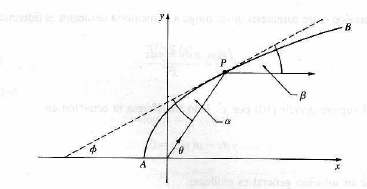
\includegraphics[scale=.4]{imagenes/espejo.png}
\end{center}
\caption{Reflejo en un espejo curvo}
\end{wrapfigure}
 \textbf{Solución.} Sea $(x,y)$ el punto de incidencia. Apelando a la geometría elemental, $\phi=\beta$ y $\theta=\alpha+\phi=2\beta$. Como $\tan\theta=\frac{y}{x}$
  y como
  \[\tan\theta =\tan 2\beta=\frac{2\tan\beta}{1-\tan^2\beta},\]
deducimos que
\[\frac{y}{x}=\frac{2 dy/dx}{1-(dy/dx)^2}.\]
Despejando
\[\frac{dy}{dx} =\frac{-x\pm\sqrt{x^2+y^2}}{y}.\]

Que es la familia de todas las parábolas con eje de simetría $x$, positivamente orientadas y con foco en $(0,0)$.
 \begin{wrapfigure}[11]{r}{5cm}
 \begin{center}
 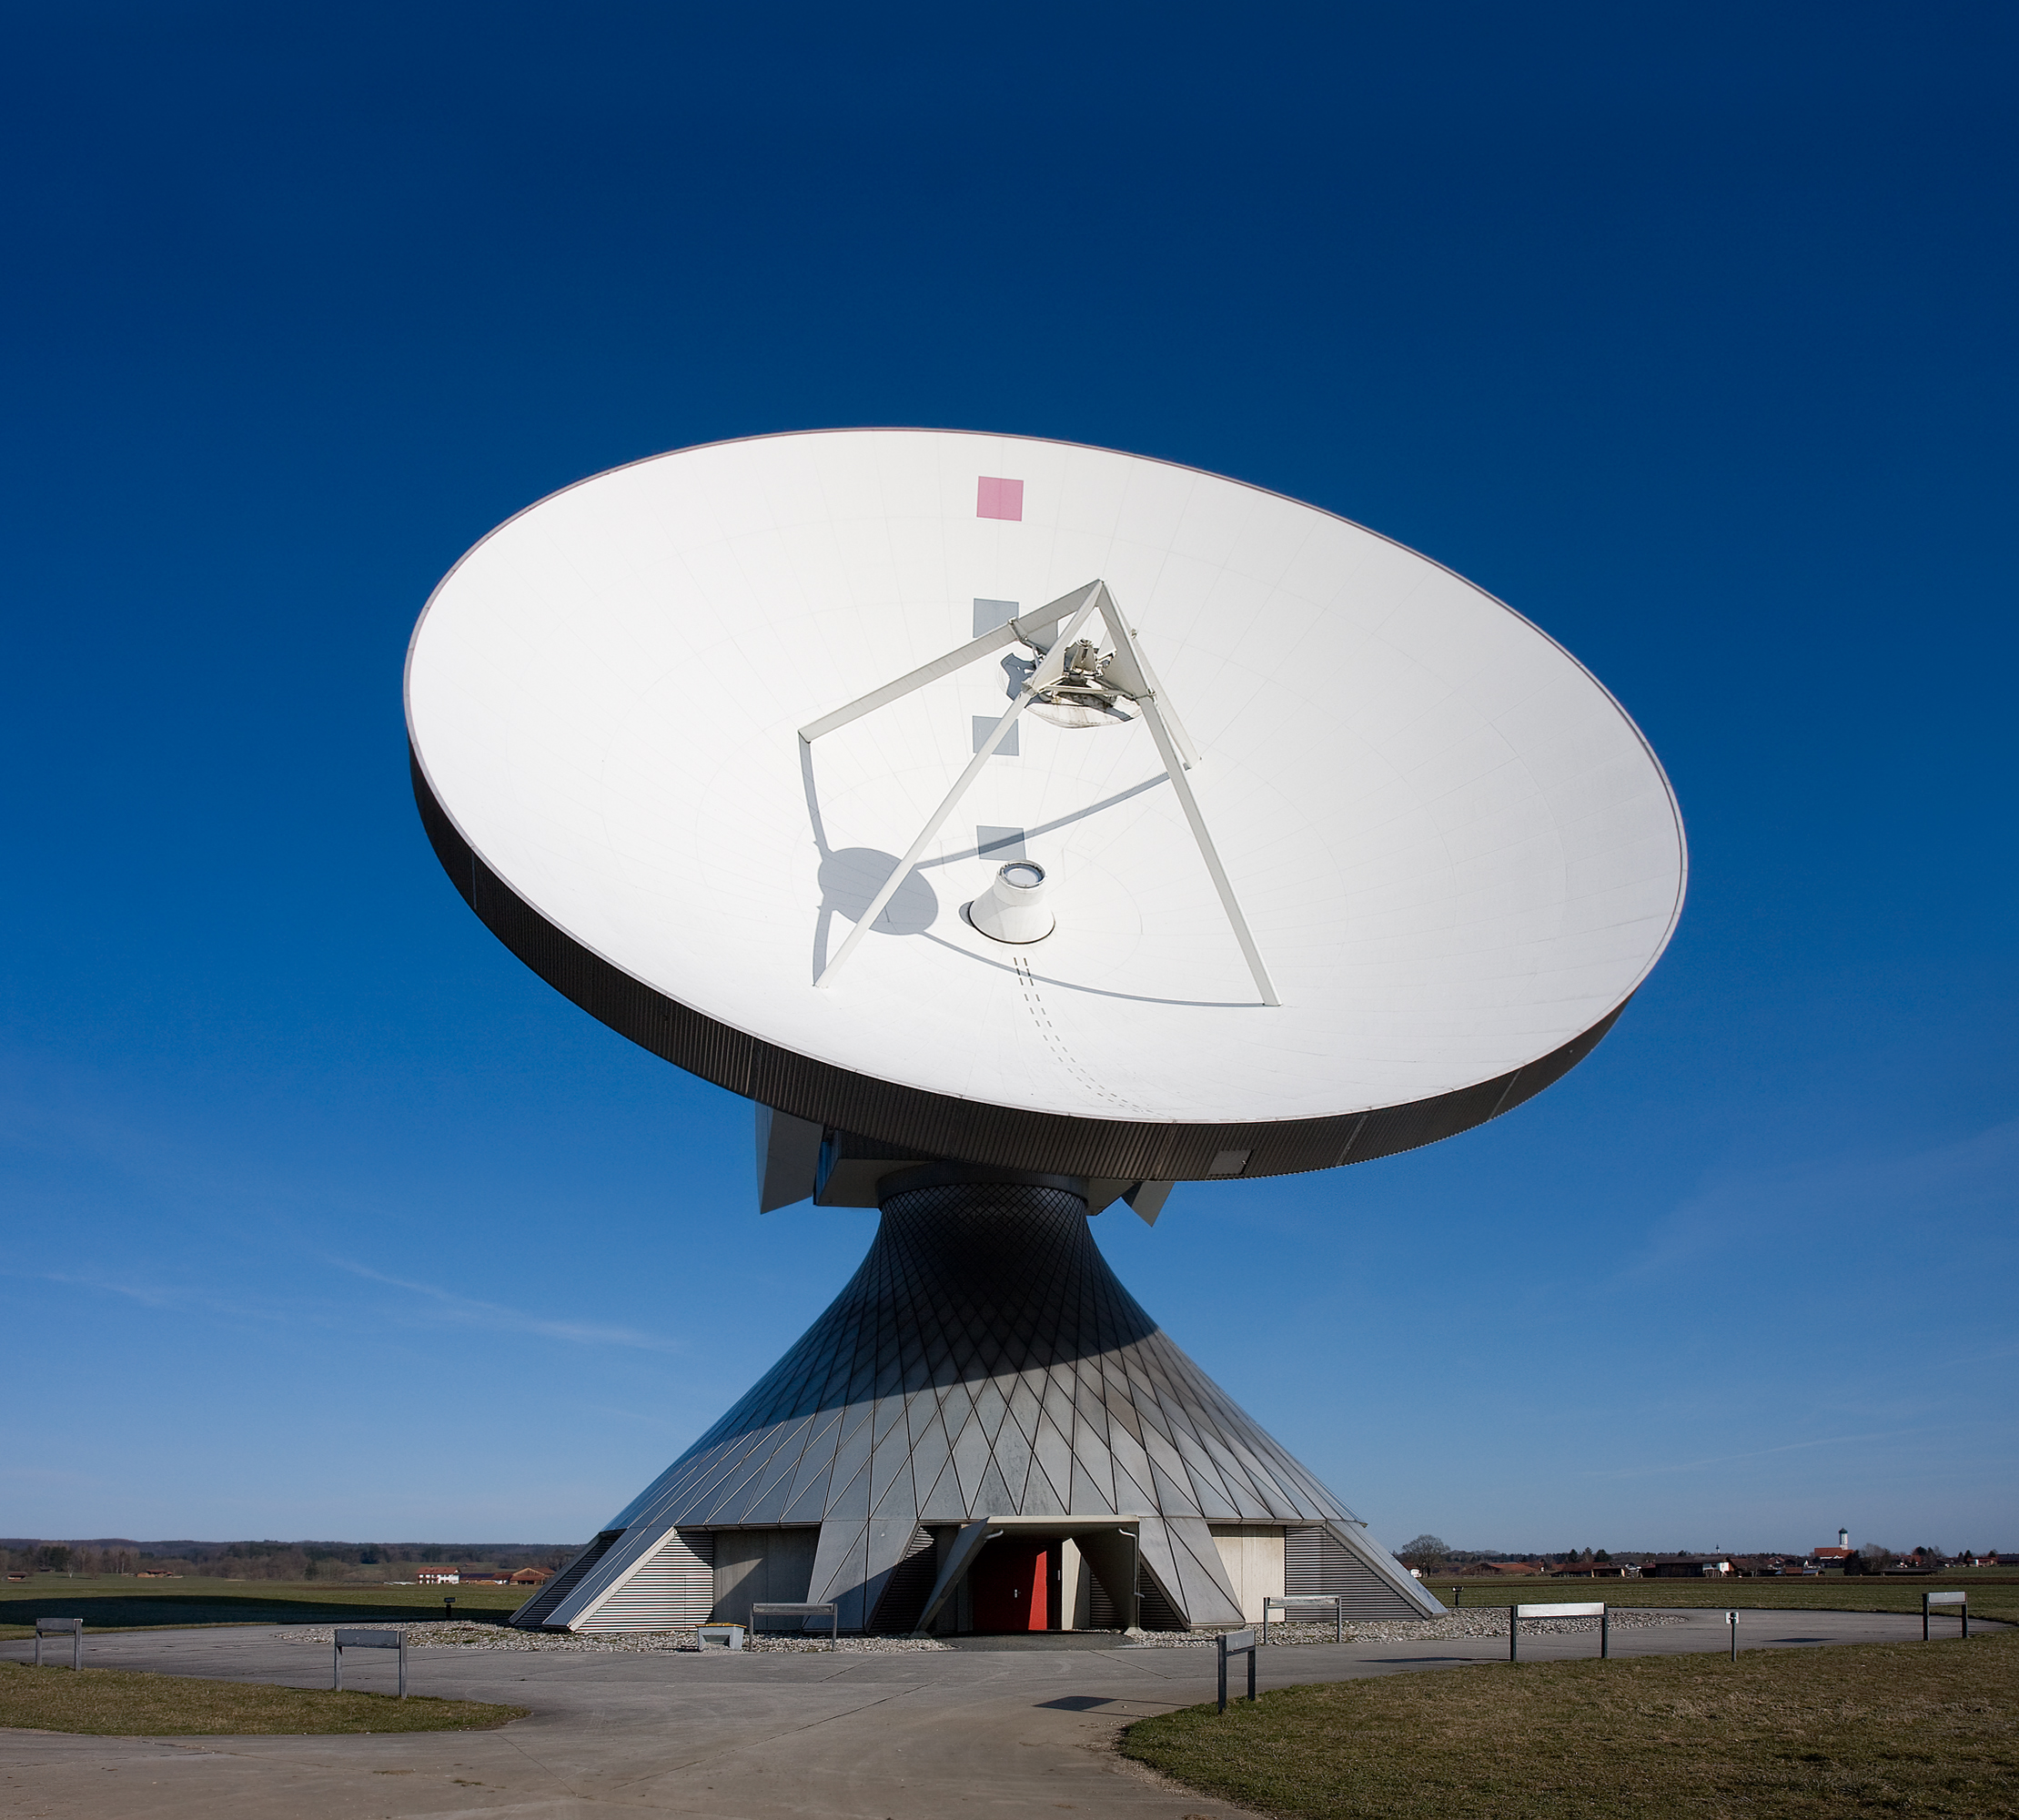
\includegraphics[scale=.1]{imagenes/antena.jpg}
 \end{center}
\caption{Antena parabólica}
\end{wrapfigure}
Podemos escribir la ecuación de este otro modo
\[xdx+ydy=\pm\sqrt{x^2+y^2}dx.\]
Tomando en cuenta \eqref{eq:exacta_mod2}
\[\pm\frac{d(x^2+y^2)}{2\sqrt{x^2+y^2}}=dx.\]
Si $r=x^2+y^2$
\[dx=\pm\frac{dr}{2\sqrt{r}}=\pm d\sqrt{r}=\pm d\sqrt{x^2+y^2}\]
Las solución general es
\[\pm\sqrt{x^2+y^2}=x+c.\]
Elevando al cuadrado ambos miembros
\[y^2=2xc+c^2=2c\left(x+\frac{c}{2}\right)\]
\section{Ecuaciones Lineales}
\begin{definicion}[Ecuación lineal] Se llama \href{http://es.wikipedia.org/wiki/Ecuación_diferencial_lineal}{ecuación diferencial lineal} a una ecuación que es lineal
respecto a   la/s variables
dependientes. La siguiente es la ecuación diferencial lineal general de primer orden
%\begin{equation}\label{eq:lineal}y'+p(x)y=q(x).
\boxedeq{y'+p(x)y=q(x)}{eq:lineal}
%\end{equation}
y la  de segundo orden
\boxedeq{y''+p(x)y'+q(x)y=r(x).}{eq:lineal_orden2}
Aquí $p,q$ y $r$ son funciones de $x$ usualmente definidas sobre un intervalo abierto de $\rr$.
\end{definicion}
La ecuación puede ser no lineal repecto a la variable independiente.

Es costumbre introducir los operadores  diferenciales $L_1[y]=y'+py$  y $ L_2[y]=y''+py'+qy$.
Para una ecuación lineal, los operadores $L_1$ y $L_2$ son lineales. Es decir, $L_1[y_1+y_2]=L_1[y_1]+L_1[y_2]$.


 Vamos a resolver la ecuación lineal de primer orden \eqref{eq:lineal}. Esto es sencillo pues la forma diferencial asociada
 \begin{equation}\label{eq:lineal2}dy+(p(x)y-q(x))dx=0
  \end{equation}
tiene un factor integrante que depende sólo de $x$. En efecto como $M=p(x)y-q(x)$ y $N=1$.
 \[\frac{\mu'}{\mu}=\frac{\partial M/\partial y-\partial N/\partial x}{N}=p(x).\]
 Entonces $\mu(x)=e^{\int pdx}$ es factor integrante. Luego si multiplicamos por $\mu$ en \eqref{eq:lineal2},  la expresión  es exacta. 
 \[e^{\int pdx}dy+p(x)e^{\int pdx}ydx=q(x)e^{\int pdx}dx.\]
Podemos identificar rápidamente, sin necesidad de hacer cálculos, el correspondiente potencial.
 \[d\left(e^{\int pdx}y\right)=d\left(\int q(x)e^{\int p} dx \right).\]
Integrando
\[e^{\int pdx}y=\int e^{\int pdx}q(x)dx+C.
 \]
Entonces
 \boxedeq{y=e^{-\int pdx}\left\{\int e^{\int pdx}q(x)dx+C\right\} }{SolGenLin}
 

\begin{ejemplo} Resolver $y'+y/x=3x$.
 \end{ejemplo}


\noindent\textbf{Solución.} En la práctica, para evitar recordar fórmulas, se suele repetir el procedimiento que llevo a la fórmula \eqref{SolGenLin}, ahora, dado la cercanía
de su derivación, vamos a usarla  de manera directa. La solución general es

\[\begin{split} y(x)&=e^{-\int\frac{1}{x}dx}\left\{\int e^{\int\frac{1}{x}dx}3xdx+C\right\}\\
   &=\frac{1}{|x|}\left\{\int |x| 3xdx+C\right\}\\
   &=x^2+\frac{C}{|x|}\\
   &=x^2+\frac{C}{x}\\
  \end{split}
\]
 



\section{Reducción de orden}

Algunas ecuaciones de segundo orden
\boxedeq{F(x,y,y',y'')=0}{Gen2Or}
se pueden reducir a una de primer orden. Por ejemplo si $F$ no depende de $y$. Es decir la ecuación es
\boxedeq{F(x,y',y'')=0}
Aquí introducimos la nueva variable dependiente $\boxed{p=y'}$, que resuelve
\[F(x,p,p')=0.\]
Que es una ecuación de primer orden. Supuesto que la podemos resolver y encontrar una solución general para  $p$, tendremos
 \boxedeq{y=\int pdx+C}
Es la solución general de la ecuación de segundo orden.


Si la ecuación general de segundo orden \eqref{Gen2Or} no depende de $x$, es decir tenemos
\boxedeq{F(y,y',y'')=0}
entonces nuevamente usaremos $\boxed{p=y'}$ como nueva variable depeniente
pero también  $\boxed{y}$ como nueva variable independiente. Como
\[y''=p'=\frac{dp}{dx}=\frac{dp}{dy}\frac{dy}{dx}=\frac{dp}{dy}p\]
La ecuación se reduce a la siguiente ecuación de primer orden
\boxedeq{F\left(y,p,\frac{dp}{dy}p\right)=0}{RedOrdSinInd}



\section{\texttt{SymPy}}



\begin{codigo}[Clasificación de EDO]
\textbf{Sintaxis:} \verb+classify_ode(Eq)+

\verb+Eq+:  ecuación.

\end{codigo}
El output son los métodos que se le pueden aplicar
\begin{lstlisting}
from sympy import *
x=symbols('x')
y=Function('y')(x)
classify_ode(y.diff()+y)
\end{lstlisting}
\noindent\textbf{Resultado:}

\verb+('separable', '1st_exact','1st_linear',+

\verb+'almost_linear','1st_power_series','lie_group',+


\verb+'nth_linear_constant_coeff_homogeneous', +

\verb+'separable_Integral', '1st_exact_Integral',  +

\verb+'1st_linear_Integral','almost_linear_Integral')+

\begin{lstlisting}
Ecuacion=Eq((x**2*y-x)*sin((y.diff(x,1)))**3\
+y**5+x**3*sin(y),0)
classify_ode(Ecuacion)
\end{lstlisting}

El único método que puede aplicar \texttt{SymPy} a la ecuación 

\[(x^ 2y-x)\sen^ 3(y')+y^ 5+x^3\sen(y)=0,\]
es \verb+('lie_group',)+
\begin{lstlisting}
dsolve(Ecuacion,y)
\end{lstlisting}
 \noindent\textbf{Resultado:} Piensa, piensa   pero no llega a nada.

\begin{lstlisting}
>>>Ecuacion=Eq(y.diff()+(-x+sqrt(x**2+y**2))/y,0)
>>>classify_ode(Ecuacion)
('1st_homogeneous_coeff_best', 
'1st_homogeneous_coeff_subs_indep_div_dep', 
'1st_homogeneous_coeff_subs_dep_div_indep', 
'1st_power_series', 'lie_group', 
'1st_homogeneous_coeff_subs_indep_div_dep_Integral', 
'1st_homogeneous_coeff_subs_dep_div_indep_Integral')
\end{lstlisting}

\begin{lstlisting}
>>>dsolve(Ecuacion,y,hint='lie_group')
\end{lstlisting}

 \noindent\textbf{Resultado:} Piensa rato largo y:
\begin{lstlisting}
The given ODE (-x + sqrt(x**2 + y(x)**2))/y(x) + Derivative(y(x), x) 
cannot be solved by the lie group method
\end{lstlisting}


\begin{lstlisting}
>>>sol=dsolve(Ecuacion,y,hint='1st_homogeneous_coeff_best')
\end{lstlisting}

\[y{\left (x \right )} = C_{1} e^{\int^{\frac{x}{y{\left (x \right )}}} -\frac{u_{2}}{u_{2}^{2} - u_{2} \sqrt{u_{2}^{2} + 1} - 1}\, du_{2} + \int^{\frac{x}{y{\left (x \right )}}} \frac{\sqrt{u_{2}^{2} + 1}}{u_{2}^{2} - u_{2} \sqrt{u_{2}^{2} + 1} - 1}\, du_{2}}\]



\section{Ejemplos}


\subsection{Velocidad de escape}\label{pag:vel_esc}



\begin{problema}[Velocidad de escape] Que velocidad hay que imprimirle a un proyectil que es lanzado verticalmente desde la superficie de la Tierra si nuestra pretensión
es que el proyectil se escape al infinito. La velocidad más chica con esta cualidad se llama 
\href{http://es.wikipedia.org/wiki/Velocidad_de_escape}{velocidad de escape}.
\end{problema}

\begin{wrapfigure}[11]{r}{5cm}
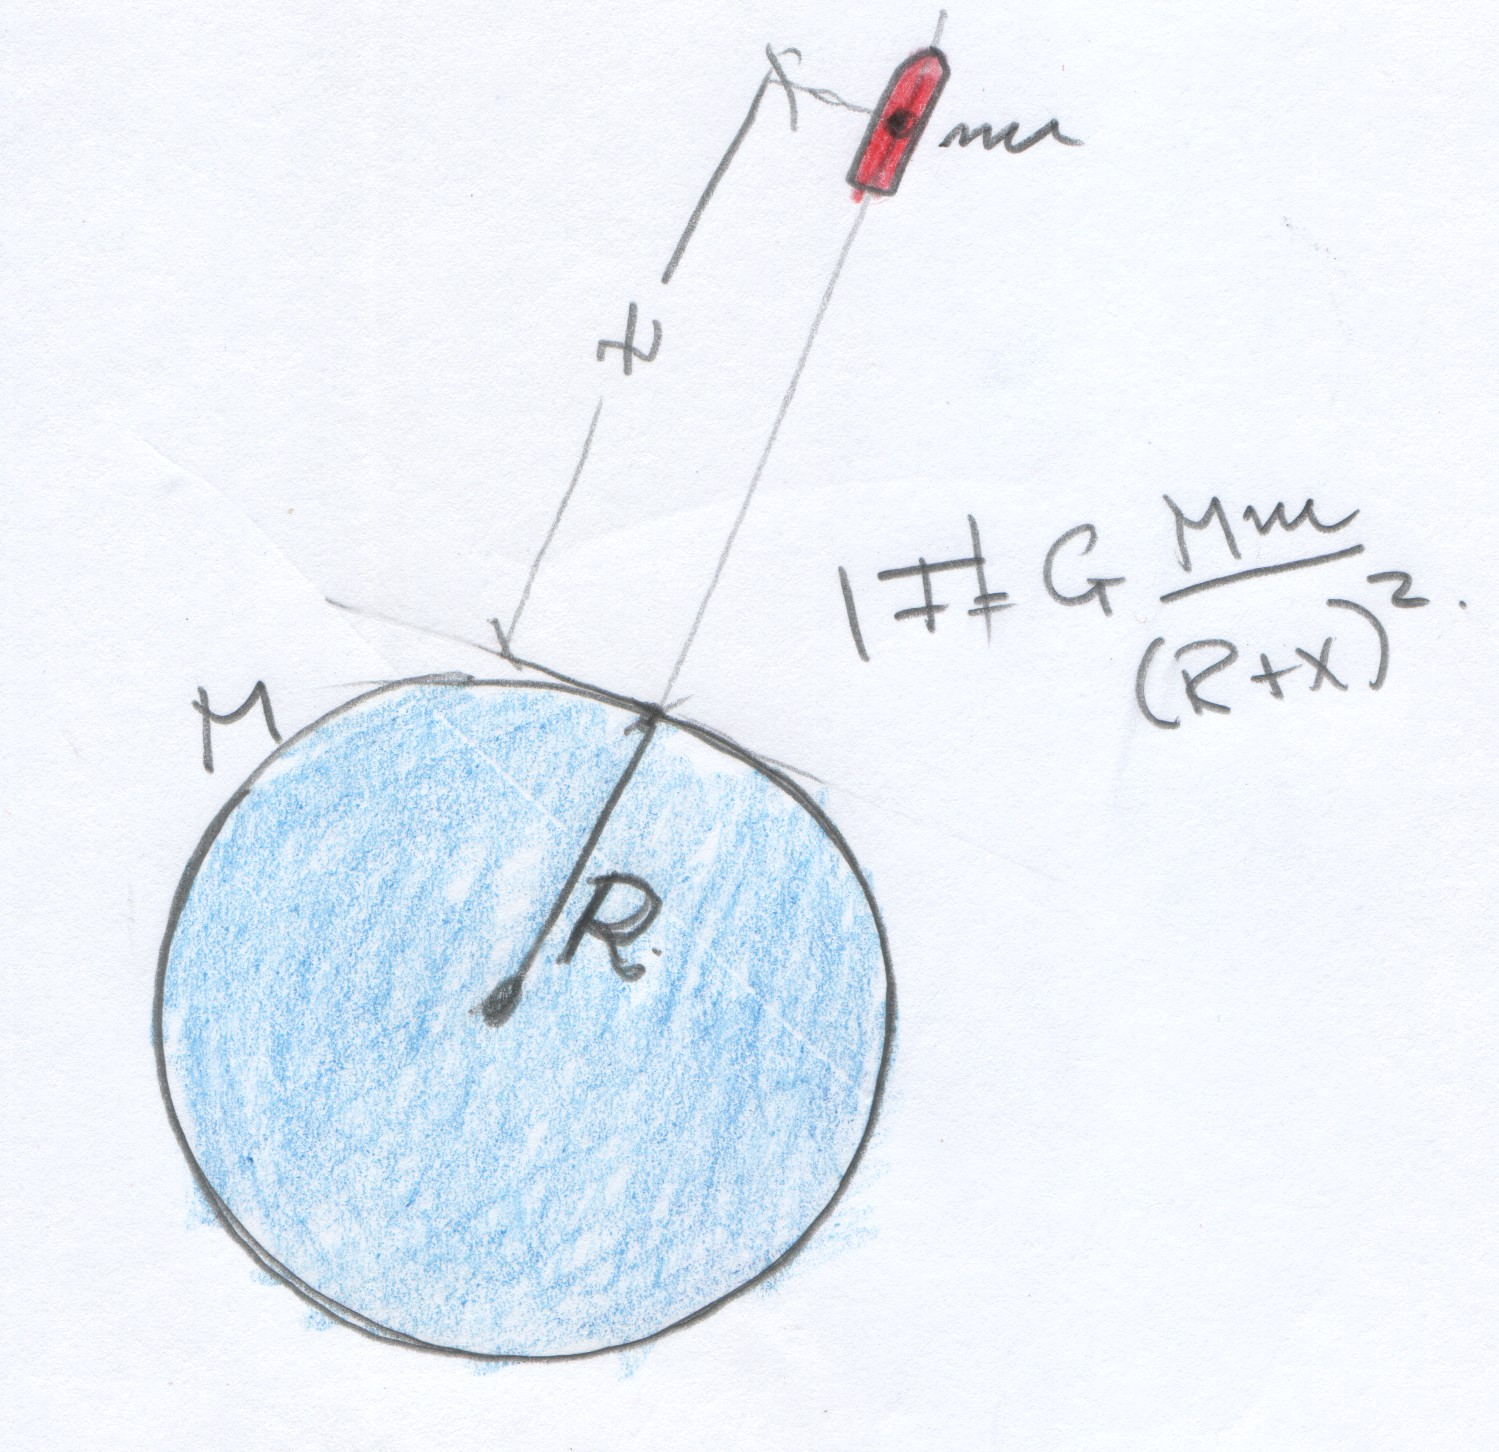
\includegraphics[scale=.075]{imagenes/tiro_vertical.jpg}
\end{wrapfigure}
 \noindent\textbf{Solución.} Para resolver este problema hay que tomar en consideración la
\href{http://es.wikipedia.org/wiki/Ley_de_gravitación_universal}{Ley de gravitación universal} de Newton. En la parte que nos interesa, esta Ley afirma
que el módulo de la fuerza de gravedad que se ejercen entre si dos cuerpos de masa $m_1$ y $m_2$ separados una distancia $r$ es proporcional al producto de las masas  
e inversamente proporcional al cuadrado de las distancia que los separa. Vale decir
\[|F|=G\frac{m_1m_2}{r^2},\]
donde $G$ es la constante de proporcionalidad.
Cuando los cuerpos no son puntos masa, sino cuerpos extendidos en el espacio, la distancia de separación hay que medirla entre los centros de masa de los cuerpos. 



Hay que aclarar que usando el \href{https://docs.google.com/file/d/0B80iJ0HgObRRWll6MlJFSjFNMGc/edit}{Principio conservación energía mecánica} podemos resolver
el problema de una manera más simple. Incluso podemos ver que la suposición de que el tiro es vertical no es necesaria, es decir la velocidad de escape es la misma aunque
el tiro sea oblicuo. Discutiremos esa solución durante la clase. Lamentablemente,  esta solución no usa ecuaciones diferenciales.
Vamos a dar una solución, quizás un poco más complicada, pero que invoca las técnicas 
discutidas.

 
Supondremos a la Tierra una esfera de radio $R$, masa $M$ y su centro de masa en el centro de la esfera.   Al proyectil lo supondremos un punto masa 
con masa $m$ y su posición en el momento $t$, denotada $x=x(t)$, la mediremos sobre un eje vertical con origen en la superficie de la Tierra.  Todo como está indicado en la página \ref{pag:vel_esc}. 
Luego la distancia Tierra-proyectil será igual a $R+x$ donde $x$ es la posición del proyectil. Utilizando la \href{http://es.wikipedia.org/wiki/Leyes_de_Newton\#Segunda_ley_de_Newton_o_ley_de_fuerza}{Segunda ley de Newton}, $F=ma$, obtenemos
\[mx''(t)=-\frac{GMm}{(R+x)^2}.\]
Es una ecuación de la forma
\[F(t,x,x',x'')=0.\]
Con variable dependiente $x$ e independiente $t$. Pero, en realidad no depende de $t$ y por consiguiente, como vimos, se puede convertir en una ecuación de primer orden
tomando como nuevas variables: 1) independiente $x$ 2) dependiente $v=x'$. En estas variables
\[\frac{d^2x}{dt^2}=\frac{dv}{dt}=\frac{dv}{dx}\frac{dx}{dt}=v\frac{dv}{dx}.\]
La ecuación se convierte en
\[v\frac{dv}{dx}=-\frac{GM}{(R+x)^2}\Longrightarrow vdv+\frac{GM}{(R+x)^2}dx=0.\]
Que es una ecuación en variables separables y también es exacta. Usaremos la técnica discutida para 
ecuaciones exactas \footnote{Siempre las ecuaciones en variables separables son exactas pues se escriben de la forma
\[M(x)dx+N(y)dy=0,\]
por consiguiente tienen potencial
\[f=\int M(x)dx +\int N(y)dy\]}, los que nos indica que la solución general se expresa de la siguiente forma
\begin{equation}\label{energia}
 \frac{v^2}{2}-\frac{GM}{(R+x)}=E=\text{cte}.
\end{equation}

\begin{wrapfigure}[12]{r}{5cm}
\begin{center}
 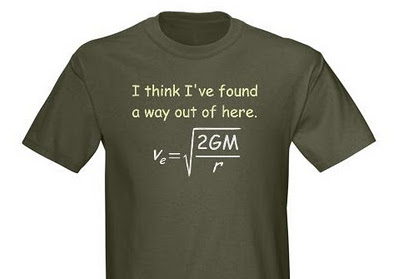
\includegraphics[scale=.3]{imagenes/velocidad_escape.jpg}
\end{center}
\caption{Remera nerd}\label{fig:vel_escape}
\end{wrapfigure}
La igualdad anterior es precisamente  consecuencia directa del \href{https://docs.google.com/file/d/0B80iJ0HgObRRWll6MlJFSjFNMGc/edit}{Principio conservación energía mecánica}, lo hemos vuelto a deducir como consecuencia de que la ecuación era exacta.  Sea $v_0$ la velocidad inicial para $t=0$. Como $E$ es constante y $x=0$ en $t=0$ debemos tener
\begin{equation}\label{energia_cero}
 E=\frac{v_0^2}{2}-GM/R
\end{equation}
Como $v^2\geq 0$ y por \eqref{energia} y \eqref{energia_cero}.
\[-\frac{GM}{(R+x)}\leq\frac{v^2}{2}-\frac{GM}{(R+x)}=\frac{v_0}{2}-\frac{GM}{R}\]
Queremos encontrar $v_0$ tal que $x\to\infty$. Luego tiene sentido tomar límite cuando $x\to\infty$ en la expresión anterior y concluimos
\[0\leq \frac{v_0^2}{2}-GM/R\]
De aquí deducimos que el valor mínimo de velocidad de escape es el impreso en la remera de la figura \ref{fig:vel_escape}.

\subsection{Curvas de persecución}
 
\begin{problema}[Curvas de persecución] Supongamos que un conejo se mueve sobre una
línea recta con rapidez uniforme $a$ y de un punto por fuera de la recta parte un perro que lo 
persigue con rapidez uniforme $b$. Encontrar la trayectoria del perrro.
\end{problema}

\begin{figure}[h]
\begin{center}
\animategraphics[controls, scale=.4]{15}{pursuit/pursuit-}{0}{40}
 \caption{\small Persecución en un pentágono estrellado.
\href{https://www.sciencenews.org/article/art-pursuit-3}{Art of Pursuit},
Ivars Peterson
}
\end{center}
\end{figure}

\begin{wrapfigure}[12]{r}{5cm}
\begin{center}
\vspace{-1cm}
 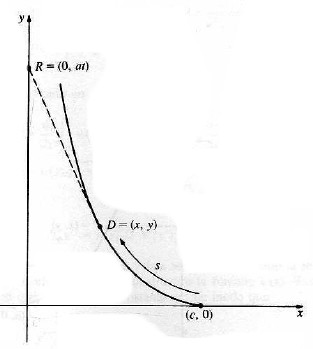
\includegraphics[scale=.3]{imagenes/persecucion.jpg}
\end{center}
\caption{Curva persecución}\label{fig:curva_per}
\end{wrapfigure}
Supongamos que el perro parte del punto $(c,0)$, el conejo de $(0,0 )$ y la recta sobre la cual se mueve el conejo en dirección positiva  es el eje $y$. 
Vamos a suponer que la trayectoria del perro sigue la trayectoria donde
la tangente a su movimiento, en un momento dado, intersecta a la posición del conejo correspondiente a ese momento.


Pasado un tiempo $t$, el conejo estará en el punto $(0,at)$ y el perro en un punto de su trayectoria que forma un arco de
 longitud $s=bt$ hasta el $(c,0)$. Ese punto, donde está el perro, lo denotaremos $(x,y)$. Como hemos supuesto que la tangente a la trayectoria del perro en $(x,y)$ pasa 
 por la posición del conejo $(0,at)$ se debe cumplir que
 \begin{equation}\label{eq:persec}\frac{dy}{dx}=\frac{y-at}{x}\Longrightarrow xy'-y=-at.\end{equation}
 En esta ecuación hay tres variables, $t$ , $x$ e $y$. No hemos definido cuales son independiente y cuales depenientes.   Generalmente el tiempo $t$ se considera  variable  indepeniente, pero en la expresión de arriba aparece la derivada de $y$ respecto a $x$.
 Claramente deberíamos eliminar una de las variables. Conviene eliminar $t$, dado que al no aparecer en la derivación no tendremos que hacer un cambio de variables allí, donde siempre es un poco más engorroso.   Por otra parte, la intuición del problema, nos dice que  a cada $t$ corresponde uno, y sólo un, $x$\footnote{De lo contrario el perro no se hubiera movido en la dirección horizontal entre dos moementos, lo que es absurdo}, lo que indica que $t$ es función de $x$ y por consiguiente es de esperar poder escribir la ecuación \eqref{eq:persec} en términos de $x$ e $y$.   Tener en cuenta que no es  razonable en matemática, como en la política,  pensar que lograremos tener un beneficio (menos variables) sin pagar algún precio, pues, como dice el dicho,
 ``Cuando la limosna es grande hasta el santo desconfía'' .
 En este caso, el costo que pagaremos 
 es incrementar el orden de la ecuación. 
 Como hemos dado algunas técnicas de  resolver ecuaciones de orden dos quizás estemos en condiciones de pagar este precio.
 
Para eliminar $t$ de la ecuación derivamos $\eqref{eq:persec}$ respecto a $x$, obtenemos
\[xy''=-a\frac{dt}{dx}.\]
Como $ds/dt=b$ 
\[\frac{dt}{dx}=\frac{dt}{ds}\frac{ds}{dx}=-\frac{\sqrt{1+y'(x)^2}}{b}.\]
Hemos usado la relación $s=\int_x^c\sqrt{1+y'^2}dx$.
 Entonces 
 \boxedeq{xy''=\frac{a\sqrt{1+y'(x)^2}}{b}.}

Que es una ecuación que no contiene $y$. De modo que usando $p=y'$ como variable dependiente reducimos el orden de la ecuación. Nos queda
\[\frac{dp}{\sqrt{1+p^2}}=\frac{a}{b}\frac{dx}{x}.\]
Que es una ecuación en variable separables. Tomando la integral definida entre $c$ y $x$, y considerando que si $x=c$ entonces $p=0$, tenemos
\[\ln\left(p+\sqrt{1+p^2}\right)=\ln\left( \frac{x}{c}\right)^{\tfrac{a}{b}}.\]
 Si despejamos $p$ conseguimos
 \boxedeq{p=\frac{dy}{dx}=\frac{1}{2}\left[\left(\frac{x}{c}\right)^{a/b}-\left(\frac{c}{x}\right)^{a/b}\right].}
Para hhalar $y$ hay que recordar que $y'=p$ e $y(1)=0$.

Usemos \texttt{SymPy} para completar este cálculo y hacer los gráficos. El siguiente código evalúa la integral, halla la constante de integración para que $y(1)=0$ y grafica.

\begin{lstlisting}
from sympy import *
x=symbols('x',real=True)
a=Rational(2)
b=Rational(1)
c=Rational(1)
y=integrate((x/c)**(a/b)-(c/x)**(a/b),x)
C=symbols('C')
C=solve(y.subs(x,1)+C,C)[0]
plot(y+C,(x,0.001,1))
\end{lstlisting}

Los resultados son:

\begin{tabular}{m{5cm} m{5cm}}
\begin{center}
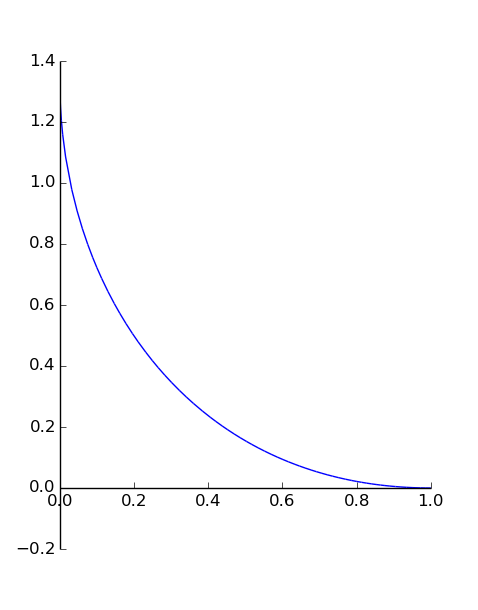
\includegraphics[scale=.3]{imagenes/perse_a_1_b_2.png}

$a<b$
\end{center}
&
\begin{center}
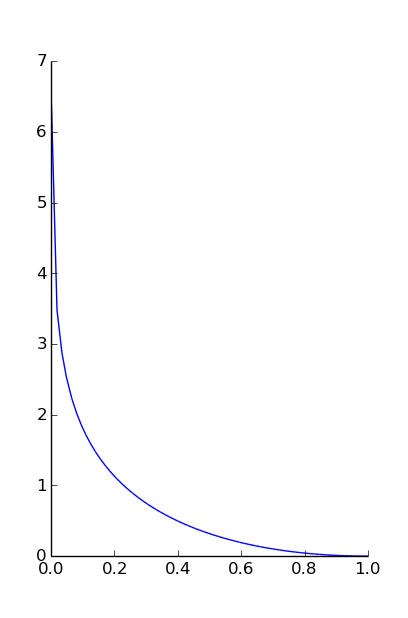
\includegraphics[scale=.3]{imagenes/perse_a_1_b_1.png}

$a=b$
\end{center}
\end{tabular}
\begin{center}
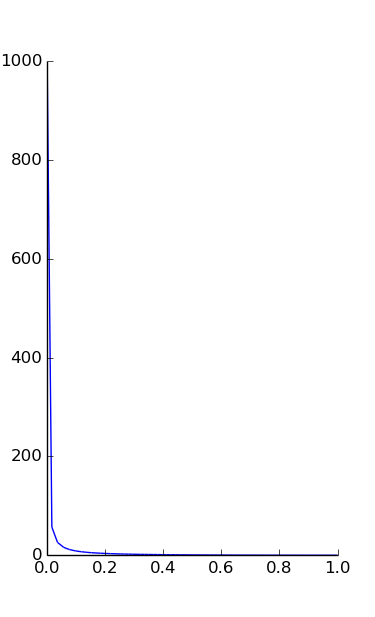
\includegraphics[scale=.3]{imagenes/perse_a_2_b_1.png}

$a>b$
\end{center}


\begin{wrapfigure}[10]{r}{6cm}
\begin{center}
 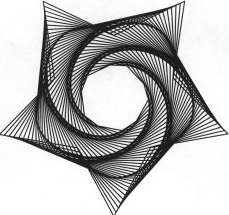
\includegraphics[scale=.4]{imagenes/persecucion2.jpg}
 \caption{\small Persecución en un pentágono estrellado.
\href{https://www.sciencenews.org/article/art-pursuit-3}{Art of Pursuit},
Ivars Peterson
}
\end{center}
\end{wrapfigure}
Lo anterior constituye un ejemplo de lo que se conoce como \href{https://en.wikipedia.org/wiki/Pursuit_curve}{curva de persecución}. Este es un tema muy interesante que tiene varias generalizaciones, por ejemplo el \href{https://en.wikipedia.org/wiki/Mice_problem}{problema de los ratones} donde se colocan en cada vértice de un polígono ratones cada uno de los cuales persigue al vecino en sentido antihorario (u horario, da lo mismo). Se consiguen patrones geométricos myu bellos




\section{Oscilador armónico}\label{resortito}



\begin{wrapfigure}[12]{r}{5cm}
\begin{center}
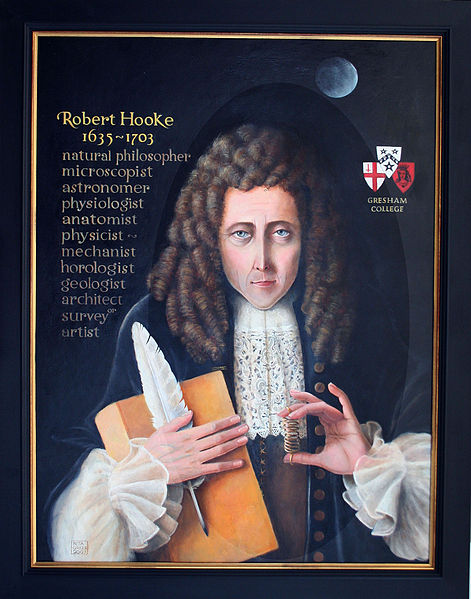
\includegraphics[scale=.15]{imagenes/Hooke.JPG}\\
\caption{Robert Hooke}
\end{center}
\end{wrapfigure}
Un \href{http://es.wikipedia.org/wiki/Oscilador_armónico}{oscilador armónico} es el más simple de los sistemas físicos vibratorios. Podemos definirlo como un sistema
elástico que obedece a la \href{http://es.wikipedia.org/wiki/Ley_de_Hooke}{Ley de elasticidad de Hooke}, en honor a su descubridor 
\href{http://es.wikipedia.org/wiki/Robert_Hooke}{Robert Hooke}.

Suele citarse al \href{http://es.wikipedia.org/wiki/Resorte}{resorte} como un ejemplo familiar de oscilador armónico. Esto debido a que, cuando las oscilaciones de un resorte son
pequeñas,  se satisface aproximadamente la Ley de elasticidad de  Hooke. Esta ley  afirma que la fuerza que ejerce un resorte sobre una masa $m$ conectada a él por uno
de sus extremos es proporcional en magnitud al desplazamiento
del resorte desde la posición de equilibrio. Además la fuerza de elasticidad actúa en sentido opuesto al desplazamiento.

\begin{figure}[h]
 \begin{center}
  \animategraphics[controls, scale=.4]{15}{resorte/resorte-}{0}{47}
 \caption{Resorte}\label{fig:resortito}
 \end{center}
 \end{figure}

 Supongamos que tenemos un resorte, en unos de sus extremos fijado en una pared y unido a una masa $m$ por el otro extremo. Supongamos que no actúa otra fuerza 
 sobre la masa. Ver la animación de la figura \ref{fig:resortito}.  Pongamos un eje de coordenadas en la dirección del movimiento, con origen en la posición de equilibrio
 del resorte. Esta posición es el punto donde el resorte no ejerce fuerza. Supongamos que la dirección positiva es la dirección donde el resorte se expande. Denotemos 
 por $x(t)$ la posición de la masa en el momento $t$.    Entonces según la Segunda Ley de Newton y la Ley de Elasticidad de Hooke, tenemos que
 
 \boxedeq{mx''(t)=-kx(t).}{eq:resorte}
 
La constante de proporcionalidad $k$ se llama \href{http://es.wikipedia.org/wiki/Rigidez}{constante elástica}. La ecuación \eqref{eq:resorte} se denomina la
ecuación del oscilador armónico o ecuación del resorte.

La ecuación del oscilador armónico se escribe $0=f(t,x,x',x'')$, donde \linebreak $f(t,x,y,z)=kx+mz$ es independiente de $t$. Podemos intentar usar $x$ como variable
independiente y $z=x'$ como dependiente. Como vimos  $x''(t)=dz/dt=dz/dx z$. Así la ecuación queda
\[\begin{split}
   m\frac{dz}{dx}z=-kx &\Longrightarrow mzdz=-kxdx\Longrightarrow m\frac{z^2}{2}=-k\frac{x^2}{2}+C_1\\
   &\Longrightarrow z=\pm\sqrt{-\frac{k}{m}x^2+C_1}\\
   &\Longrightarrow x'(t)=\pm\sqrt{-\frac{k}{m}x^2+C_1}.\\
  \end{split}
\]
Debe ser $C_1\geq 0$ de lo contrario el dominio de la función sería vacío. Nos queda una nueva ecuación para $x'$.
Esta ecuación es en variables separables
\[ \frac{dx}{\sqrt{-\frac{k}{m}x^2+C_1}}=dt.   
\]
 Integrando
\[\begin{split}
   t+C_2 
   &=\int \frac{dx}{\sqrt{-\frac{k}{m}x^2+C_1}}\\
   &= \sqrt{\frac{1}{C_1}} \int \frac{dx}{\sqrt{-\frac{k}{C_1m}x^2+1}} \\  
   &= \sqrt{\frac{m}{k}} \int \frac{du}{\sqrt{1-u^2}}\quad \left(\text{haciendo } u=\sqrt{\frac{k}{C_1m}}x\right)\\ 
   &=\sqrt{\frac{m}{k}}\arcsen u.
  \end{split}
\]
Entonces
\[\begin{split}
    x=\frac{C_1m}{k}u &=\frac{C_1m}{k}\sen \left(\sqrt{\frac{k}{m}}(t+C_2)\right)\\
    &=\boxed{C_3\sen \sqrt{\frac{k}{m}}t+C_4\cos \sqrt{\frac{k}{m}}t}.
  \end{split}
 \]
Que es la solución general de la ecuación del oscilador armónico. Como vemos el movimiento es oscilatorio con frecuencia
\[\boxed{f=\sqrt{\frac{k}{m}} }.\]
En particular, no importan las condiciones iniciales, la frecuencia es siempre la misma. 

 
 



\section{EDP, método características}

Saber resolver ecuaciones ordinarias de primer orden nos permite resolver algunas ecuaciones en derivadas parciales de primer orden.  Vamos a exponer este punto a través del \href{https://en.wikipedia.org/wiki/Method_of_characteristics}{método de características}.

Para tener un problema bien planteado con  ecuaciones en derivadas parciales no es suficiente conocer el valor de la función en un punto (como en una EDO de primer orden). Una condición típica extra, para lograr este propósito,  es consignar el valor de la función a lo largo de una curva, que por simplicidad asumiremos que es una recta .

\begin{ejemplo}
\begin{equation}\label{eq:EDP_gral_1orden}
  \left.\begin{array}{l}
  a(x,y)u_x+b(x,y)u_y=c(x,y,u)\\
  u(x,0)=f(x)\\
\end{array}\right\}
\end{equation}
Aquí $x,y$ son variables independientes y $u$ dependiente. La primera línea es la ecución diferencial, que incluye derivadas parciales de la incognita y la segunda línea podemos denominarla condición inicial (pensando que la variable $y$ representa tiempo).
\end{ejemplo}

El método de características consiste en encotrar $u$ a lo largo de las soluciones de la EDO

\boxedeq{\frac{dy}{dx}=\frac{b(x,y)}{a(x,y)}}{eq:ecua_caract}

Una solución de esta ecuación es normalmente una curva en el plano  $x,y$. La idea es que las soluciones de \eqref{eq:ecua_caract} forman un flia uniparamétrica
 de curvas que llena una gran parte $\Omega$ del plano $x,y$.  Así terminamos conociendo el valor de $u$ sobre este conjunto $\Omega$. Para que \eqref{eq:ecua_caract} tenga sentido debemos tener $a\neq 0$. De todas formas si $a=0$ podemos invertir los roles de $x$ e $y$.

Supongamos $y(x)$ solución de \eqref{eq:ecua_caract}, entonces pongamos por abuso de notación $u(x)=u(x,y(x))$. Se tiene que

\boxedeq{\frac{du}{dx}=u_x+u_yy'=u_x+u_y\frac{b}{a}=\frac{c(x,y(x),u(x))}{a(x,y)}}{eq:ecua_caract2}
Que es otra ecuación ordinaria. Podemos escribir  \eqref{eq:ecua_caract} y \eqref{eq:ecua_caract2} en una ecuación más simétrica
\boxedeq{\frac{du}{c}=\frac{dx}{a}=\frac{dy}{b}}{eq:caract}

Estas ecuaciones se llaman \emph{ecuaciones características}. Las soluciones de estas ecuaciones son un familia de curvas que suele llenar un conjunto abierto de  $\mathbb{R}^3$.  La gráfica de la solución se obtiene eligiendo entre estas curvas las que pasan por los puntos de la gráfica de $u$ especificados en la condición inicial, es decir $(x,0,f(x))$. Esto, en los casos favorables, forma una superficie que es la gráfica de la solución. La proyección de estas curvas en el plano $x,y$ se denominan \emph{caracterísitcas}. Son la familia de soluciones de $y'=b/a$.


\begin{ejemplo} Resolver
\begin{equation}\label{eq:EDP_gral_1orden}
  \left.\begin{array}{l}
  u_x+u_y=yu\\
  u(x,0)=f(x)\\
\end{array}\right\}
\end{equation}
\end{ejemplo}
En este caso
\[\frac{dy}{dx}=\frac{b}{a}\Rightarrow y'=1\Rightarrow y(x)=x+\mu,\quad\mu=\hbox{cte}.\]
Entonces
\[\frac{du}{dx}=\frac{c}{a}\Rightarrow u'=yu=(x+\mu)u\Rightarrow \ln|u|=\frac{x^2}{2}+\mu x+C(\mu).\]
Notar que la nueva constante de integración $C(\mu)$ debe depender de la primera $\mu$. Entonces
\[u=\pm e^{\frac{x^2}{2}}e^{(y-x)x}e^{C(y-x)}.\]
Ahora
\[u(x,0)=f(x)\Rightarrow f(x)=\pm e^{\frac{x^2}{2}}e^{-x^2}e^{C(-x)}\Rightarrow C(\mu)=\frac{\mu^2}{2}+\ln|f(-\mu)|.\]
Entonces
\[u(x,y)=\pm e^{\frac{x^2}{2}}e^{(y-x)x}e^{\frac{(y-x)^2}{2}+\ln|f(x-y)|        }
=e^{\frac{y^2}{2}}f(x-y).\]





\end{document}
